%\documentclass[mathserif]{beamer}
\documentclass[handout]{beamer}
%\usetheme{Goettingen}
\usetheme{Warsaw}
%\usetheme{Singapore}
%\usetheme{Frankfurt}
%\usetheme{Copenhagen}
%\usetheme{Szeged}
%\usetheme{Montpellier}
%\usetheme{CambridgeUS}
%\usecolortheme{}
%\setbeamercovered{transparent}
\usepackage[english, activeacute]{babel}
\usepackage[utf8]{inputenc}
\usepackage{amsmath, amssymb}
\usepackage{dsfont}
\usepackage{graphics}
\usepackage{cases}
\usepackage{graphicx}
\usepackage{pgf}
\usepackage{epsfig}
\usepackage{amssymb}
\usepackage{multirow}	
\usepackage{amstext}
\usepackage[ruled,vlined,lined]{algorithm2e}
\usepackage{amsmath}
\usepackage{epic}
\usepackage{epsfig}
\usepackage{fontenc}
\usepackage{framed,color}
\usepackage{palatino, url, multicol}
\usepackage{listings}
%\algsetup{indent=2em}
\newcommand{\factorial}{\ensuremath{\mbox{\sc Factorial}}}
\newcommand{\BIGOP}[1]{\mathop{\mathchoice%
{\raise-0.22em\hbox{\huge $#1$}}%
{\raise-0.05em\hbox{\L
\usepackage{fontenc}
\usepackage{framed,color}
\usepackage{palatino, url, multicol}
\usepackage{listings}
%\algsetup{indent=2em}
\newcommand{\factorial}{\ensuremath{\mbox{\sc Factorial}}}
\newcommand{\BIGOP}[1]{\mathop{\mathchoice%
{\raise-0.22em\hbox{\huge $#1$}}%
{\raise-0.05em\hbox{\Large $#1$}}{\hbox{\large $#1$}}{#1}}}
\newcommand{\bigtimes}{\BIGOP{\times}}
\vspace{-0.5cm}
\title{Introduction to Statistical Inference}
\vspace{-0.5cm}
\author[Felipe Bravo Márquez]{\footnotesize
%\author{\footnotesize  
 \textcolor[rgb]{0.00,0.00,1.00}{Felipe José Bravo Márquez}} 
\date{ \today }
arge $#1$}}{\hbox{\large $#1$}}{#1}}}
\newcommand{\bigtimes}{\BIGOP{\times}}
\vspace{-0.5cm}
\title{Introduction to Bayesian Inference}
\vspace{-0.5cm}
\author[Felipe Bravo Márquez]{\footnotesize
%\author{\footnotesize  
 \textcolor[rgb]{0.00,0.00,1.00}{Felipe José Bravo Márquez}} 
\date{ \today }


\begin{document}
\begin{frame}
\titlepage


\end{frame}


%%%%%%%%%%%%%%%%%%%%%%%%%%%


\begin{frame}{Introduction to Statistical Thinking}
\scriptsize{
\begin{itemize}
 \item Statistical thinking is a way of understanding a complex world by describing it in relatively simple terms.
 \item The idea is to capture essential aspects of its structure and to  provide us some idea of how uncertain we are about that knowledge. 
 
 \item The foundations of statistical thinking come primarily from mathematics and statistics, but also from computer science, psychology, and other fields of study. \cite{poldrack2019statistical}
\end{itemize}

} 
\end{frame}

\begin{frame}{Motivation}

\scriptsize{
\begin{itemize}
\item Collections of data are stored on a daily basis. For example: The Web, e-commerce, transactional data.
\item Computers are becoming cheaper and more powerful.
\item Analyzing this data allows to find hidden patterns. 
\item A good use of data can bring business benefits. Ex: customer segmentation, demand prediction.
\end{itemize}

}
\begin{figure}[h!]
	\centering
	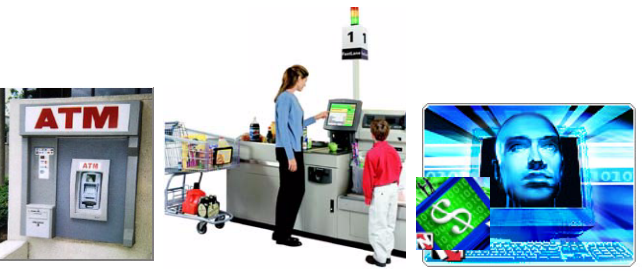
\includegraphics[scale=0.5]{pics/supermercado.png}
\end{figure}
 
\end{frame}


\begin{frame}{Probability and Statistics}

\scriptsize{
\begin{itemize}
 \item Probability is the language of uncertainty that is also the basis for statistical inference.
 \item The problem studied in probabilities is: given a data generating process, which are the properties of the outputs?
 \item The problem studied in statistical inference, data mining and machine learning is: given the outputs, what can we say about the process that generates the observed data? 
\end{itemize}

}
\begin{figure}[h!]
	\centering
	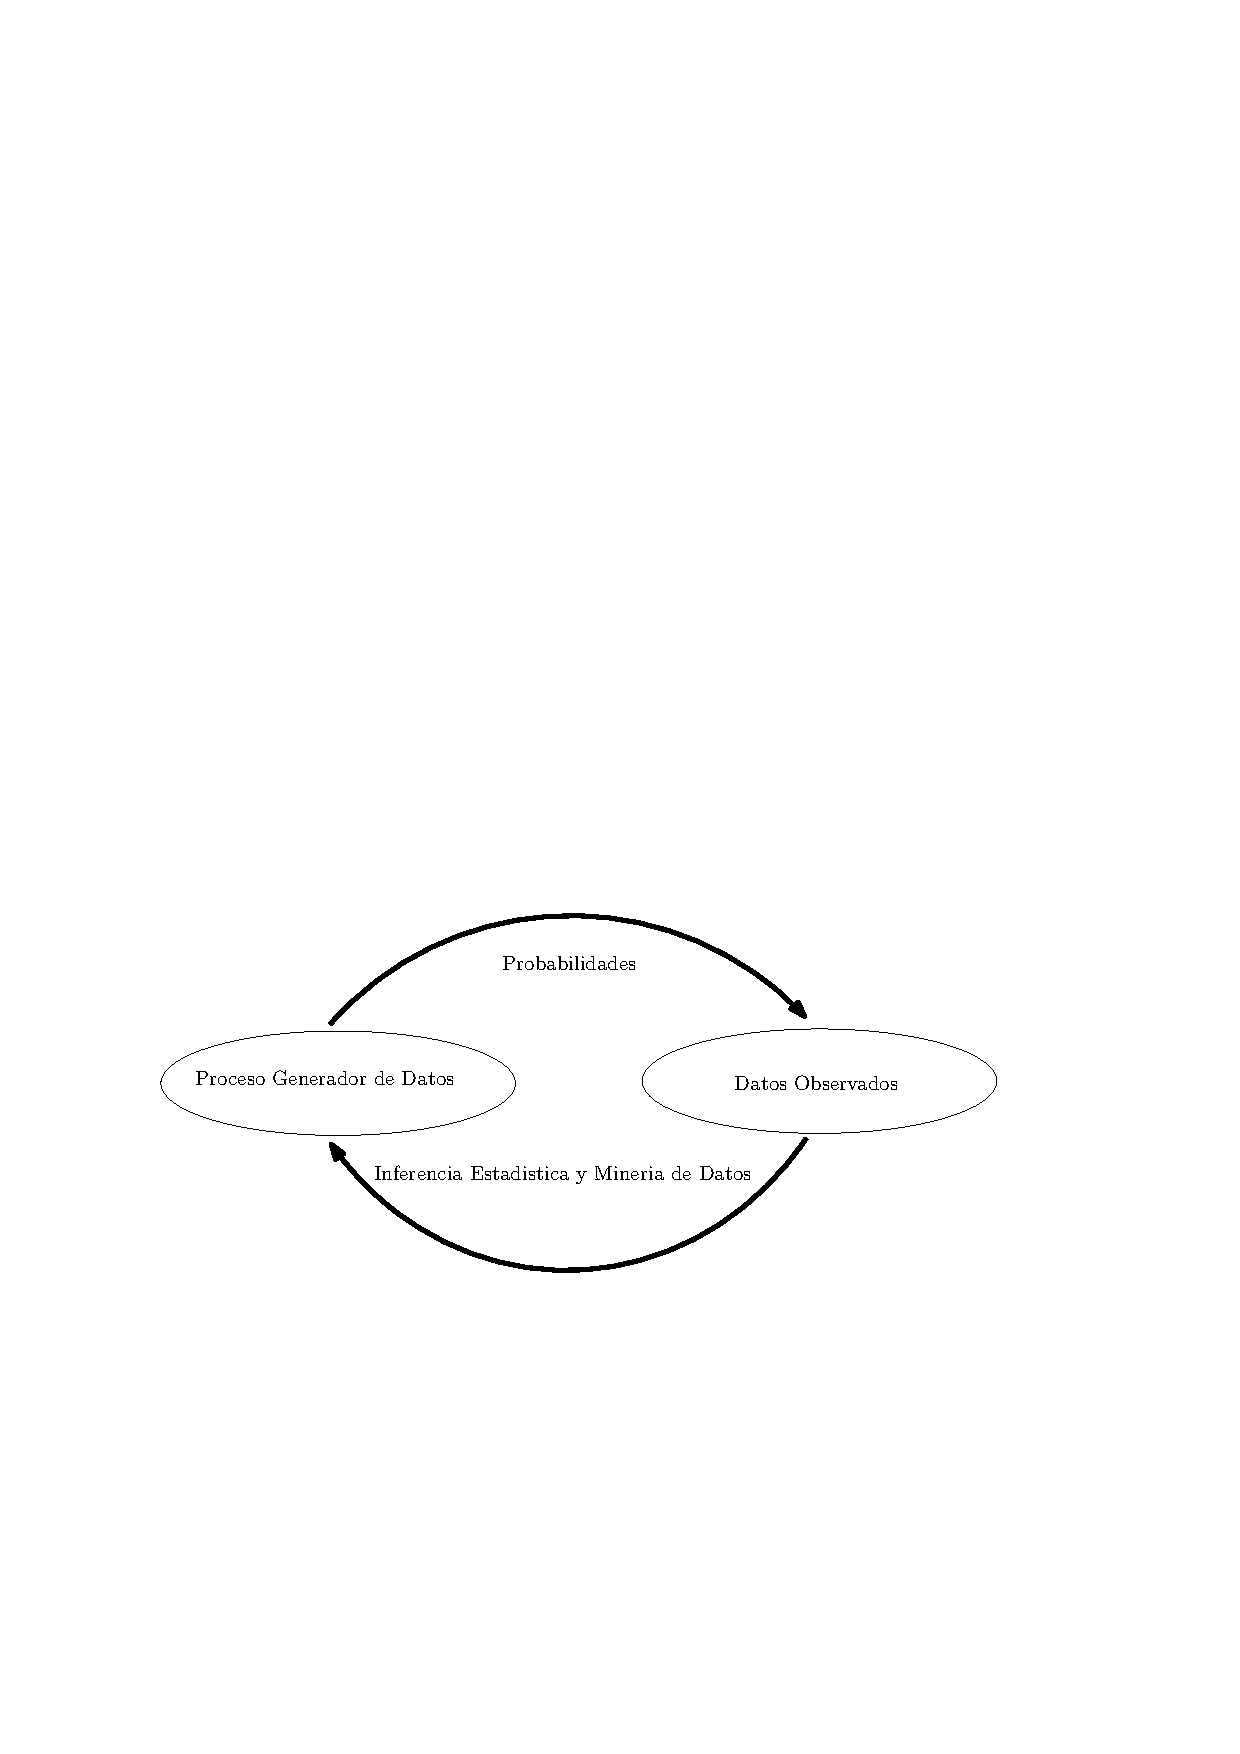
\includegraphics[scale=0.6]{pics/proceso.pdf}
\end{figure}
 
\end{frame}


%%%%%%%%%%%%%%%%%%%%%%%%%%%
\begin{frame}[allowframebreaks]\scriptsize
\frametitle{References}
\bibliography{bio}
\bibliographystyle{apalike}
%\bibliographystyle{flexbib}
\end{frame}  









%%%%%%%%%%%%%%%%%%%%%%%%%%%

\end{document}
